% !TeX spellcheck = en_US
\documentclass[11pt,a4paper,twoside,openright]{article}

\usepackage[utf8]{inputenc}
\usepackage[english]{babel}
\usepackage{amsmath}
\usepackage{mathtools}
\usepackage{amsfonts}
\usepackage{amssymb}
\usepackage{listings}  % Required for insertion of code
\usepackage{graphicx} % Required to insert images
\usepackage{textcomp}
\usepackage{enumerate} % Required for enumerate model
\usepackage{gensymb} %Required for degree symbol which is made ^{\circ}
\usepackage{caption} %used to have cool captions
\captionsetup{
	tableposition=top,
	figureposition=bottom,
	font=small,
	format=hang, 
	labelfont=bf}	%caption setup
\usepackage[protrusion=allmath]{microtype} %used to have high quality text formatting
\usepackage{graphicx,subfig,float,wrapfig,rotating,multirow,epstopdf} %high quality tables and images formatting
\usepackage{booktabs,siunitx,array,tabularx} % tables
\usepackage{amsbsy,bm,amsmath} % math

%\usepackage [ Lenny ]{fncychap}
\usepackage{longtable} % Required to put long tables

\lstset{ % Frame for Matlab code
	numbers=left, 
	numberstyle=\small, 
	numbersep=8pt, 
	frame = single, 
	language=Matlab, 
	framexleftmargin=19pt,
	breaklines}

\pagestyle{plain}

\graphicspath{{img/}} % Set graphics directory

\def\permille{\ensuremath{{}^\text{o}\mkern-5mu/\mkern-3mu_\text{oo}}} % Add symbol of per mille
\newcommand{\parallelsum}{\mathbin{\!/\mkern-5mu/\!}} % Fix parallel symbol inclination

%\makeindex

\title{	01NVSOQ -- Advanced Antenna Engineering \\
	\huge {\textsc{Assignment 4: array components}}	}

\begin{document}
\author{Amedeo Bertone (243878)\\Davide Botteon (239595)\\Enrico Maria Renzi (244028)\\
}
\maketitle 		
\tableofcontents

\section{Introduction}
The goal of this project is the realization of the Beam Forming Network able to provide the right feeding to an array of four elements which should exhibit a tapering able to shape the array factor so that the SLL is lower than -20 dB (exercise 2 of the previous assignment)..

\par\medskip
\noindent
This first part (definition of inter-element spacing and tapering) was already carried out during the previous assignment and leaded us to choose the values that we will use during the rest of the project.

\par\medskip
\noindent
In particular, the first part of the work deals with the handmade project of the BFN in order to obtain the correct power ratios for the four radiators, which are the patches we designed in the second assignment (resonance at 2.45 GHz and 120 $\Omega$ input impedance), the correct phasing, 0 in order to obtain a broadside array, and an input impedance of 50 $\Omega$. All these specs should be met at 2.45 GHz and in the largest possible band around this frequency.
\noindent
In this part, simulation of the single parts of the BFN are also provided, in order to get a glimpse on the correct or not correct behavior of the final version.

\par\medskip
\noindent
The second part is related to the simulation of the BFN. It is worth to anticipate from the very beginning that this part turned out to be very tricky, since in a first moment, through the use of \textit{CST Design Studio} we seemed to confirm our design and even optimize it in a good way, but later on we encountered lots of difficulties in replicating such results in \textit{CST Microwave Studio}, which poses lots of difficulties in the optimization due to the very long simulation time, dense meshes and huge weight of all the non linearities and non idealities. In fact, even if the single parts of our BFN work in a reasonable way when standalone, they do not work so well when they are put together. 

\par\medskip
\noindent
The third and last part deals with the simulation of the radiating structure of the array. First, a further optimization of the single patch was carried out, in order to get the most close as possible to the prescribed 120 $\Omega$ impedance and 2.45 GHz resonance. Then, the patches are put together in order to verify how they behave when assembled in order to form the array, to see how they mutually influence each other. We have to mention that even in this case simulation was not straightforward and the problems encountered in the second part about long simulation time and difficulty on tuning were present even in this case, so that the results hopefully should be, even in this case, susceptible to further perfectioning.
\section{Problem no.1}

The task is to design a corporate beam forming network that provides the correct power distribution to each radiating element. The microstrip design is carried on considering FR4 as substrate, whose technological specifications follow:

 \begin{table} [h]
 	\label{tab:p1_FR4}
 	\centering	
 	\begin{tabular}{lrrr} 
 		\toprule 
 		Quantity & Symbol & value & \\
 		\midrule
		Dielectric permittivity &$\epsilon_{r}$		&4.3		& 		\\
 		Substrate height&	h				& 1.5		&  mm	\\ 
 		Metal thickness&t	& 0.1	& mm\\
 		Minimum strip width &W\textsubscript{min}&0.15 & mm \\
 		Minimum spacing between lines &$\Delta$s\textsubscript{min}&0.175 & mm \\
 		\bottomrule 
 	\end{tabular}	
 \end{table}

The antenna's radiating part requires four radiators with cosine-over-pedestal tapering, hence the BFN is symmetric with respect to the feeding line. %What follows is the theoretical design for the network, whose final optimized solution is presented in the following section. 

One possible implementation is proposed in FIGURE* PUT FIGURE WITH BFN'S BLOCK DIAGRAM, from which it appears that the design can be divided as follows: 
\begin{description}
	\item [Splitter1] this section matches the input line to Z\textsubscript{in}=50$\Omega$ at the input port. Moreover, it evenly splits the power into the two following branches, therefore the power splitter is a 3dB splitter. 
	\item [Splitter2] this section matches the radiating elements with section1 outputs, moreover it convey power into the radiators giving the correct power ratio between elements.
	\item [Splitter3] this is symmetric to section2 with respect to the feeding line longitudinal axis. 
	\item [Match1] these lines acts as matching connection from power splitter1 to power splitters2 and 3, moreover they are used to adjust the distance between elements.
	\item [Match2] matching connections between radiators and power splitters2,33;
\end{description}
Overall the BFN must be designed in order to be compliant with:
\begin{itemize}
	\item the requirement on grating lobes, then the element spacing d (d/$\lambda_0=0.724$);
	\item the requirement on amplitude tapering between edge and centre elements;
	\item the requirement on main beam direction. Since the array is broadside then the phase shift among elements must be null.
\end{itemize}
Each block's design and simulation are reported in the following paragraphs.

\subsection{Splitter 1 design}

Figure * PUT FIGURE OF SECTION 1 PHASE,IMP shows the block diagram of splitter 1. The input line is matched to the input port by means of a 50$\Omega$ line whose length has been chosen equal to $\lambda_{g}/4$. To evenly split the power into port 2 and 3 we use a T junction made up of two quarter-wavelength transformers. This components show real input and output impedance and the following relation for their characteristic impedance holds:
\begin{equation}
	\label{eq:p1_ZcQW}
	Z_{c,QW} =R_{c,QW}=\frac{1}{G_{c,QW}}= \sqrt{R_{in,QW}\cdot R_{out,QW}} 
\end{equation}
The two quarter-wavelength transformers are seen as two parallel admittances from the input port, then to have the 50$\Omega$ matching we have:
\begin{equation}
	G_{c,QW1}+G_{c,QW2}=\frac{1}{Z_{in}}=\frac{1}{50\Omega} \; \Rightarrow \; Z_{c,QW1}=Z_{c,QW2}=Z_{c,QW}=100\Omega \notag
\end{equation}
 Willing to reduce impedance discontinuities within the network, the section's output impedance is set to 50$\Omega$ too, hence:
\begin{equation}
	Z_{c,QW}= \sqrt{R_{in,QW}\cdot R_{out,QW}}=\sqrt{100\Omega\cdot 50\Omega}=70.7\Omega \notag
\end{equation}

The design has been converted from ideal microstrip lines to physical lines by means of TX-LINE: Transmission Line Calculator (from NI AWR Design Environment) and eventually implemented in CST DS\texttrademark{} for the optimization process. The theoretical and optimized dimensions are reported in table \ref{tab:p1_sec1DimIN} and\ref{tab:p1_sec1DimIN}. The resulting scattering parameters are shown in figure \ref{fig:p1_sec1Scatt}: both power splitting and phase behaves as expected. ADD DRAWING
\begin{table} [h]
	\label{tab:p1_sec1DimIN}
	\caption{Splitter1: Input line dimensions}
	\centering	
	\begin{tabular}{lccc} 
		\toprule
			& theoretical & optimized&\\
		\midrule 
		W\textsubscript{in} 	&	3.020		&	2.964	 & mm 		\\
		L\textsubscript{in}		&	16.797		& 	17.976		& mm	\\ 
		Z\textsubscript{c,in}	& 	50 & 50.6	&$\Omega$ \\
		\bottomrule
	\end{tabular}	
\end{table}

\begin{table} [h]
	\label{tab:p1_sec1DimQW}
	\caption{Splitter1: quarter-wavelength transformer dimensions}
	\centering	
	\begin{tabular}{lccc} 
		\toprule
		& theoretical & optimized&\\
		\midrule 
		W\textsubscript{QW} 	&	1.599		&	1.458	& mm		\\
		L\textsubscript{QW}	&	17.248		& 	16.706		& mm	\\ 
		Z\textsubscript{c,QW}& 	70.7 &73.9	&$\Omega$ \\
		\bottomrule
	\end{tabular}	
\end{table}

\begin{figure}[h] 
	\centering
	\subfloat[][\emph{Modulus}]{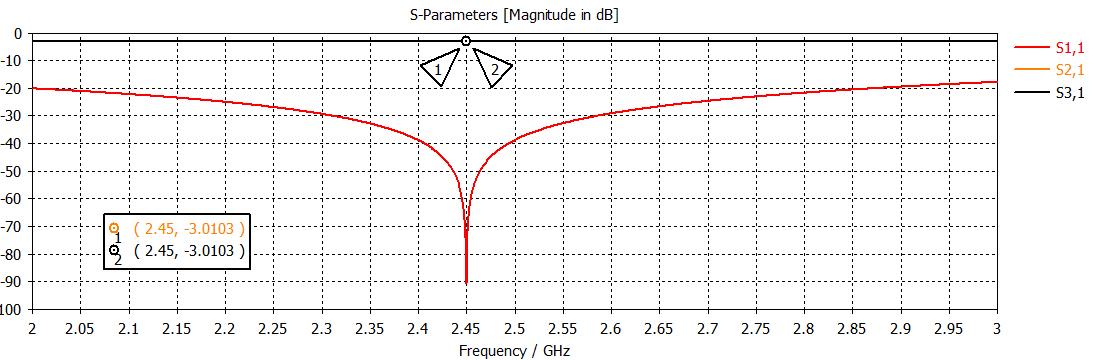
\includegraphics[scale=.6,angle=90]{p1_sec1_Smod}}\quad
	\subfloat[][\emph{Phase}]{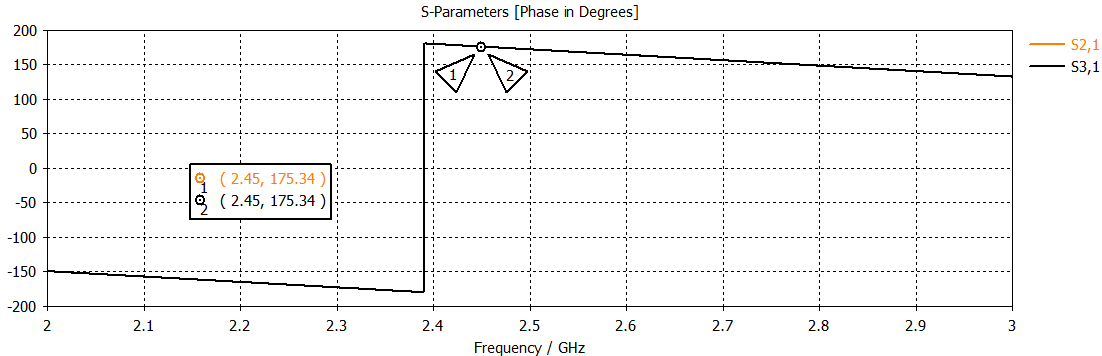
\includegraphics[scale=.6,angle=90]{p1_sec1_Sph}}\\
	\caption{Section 1 most important scattering parameters. As it appears both input matching and even power splitting are accomplished, the phase shift is null (reference impedance 50$\Omega$).}
	\label{fig:p1_sec1Scatt}
\end{figure}

\newpage

\subsection{Splitters2,3 and match2 design}

Figure * PUT FIGURE OF SECTION 2 PHASE,IMP shows the block diagram of splitter2 and match1 (splitter3  and match1 are specular).

Match1 lines are designed as $\lambda_{g}/2$, 50$\Omega$ characteristic impedance microstrip lines. Acting as transparent transmission lines, they allow splitter2 and 3 to have Z\textsubscript{in}=50$\Omega$ at their input ports. Again a Z\textsubscript{out}=50$\Omega$ is chosen to avoid abrupt impedance variations. Imposing Z\textsubscript{in}=50$\Omega$ we also avoid the appearance of lines narrower than W\textsubscript{min} within the power splitter2 (and splitter3).

The splitter is composed by two quarter-wavelength transformers that provide the correct current tapering for the radiators. To design that we will consider the power entering and exiting the component.
Having chosen as tapering t=0.54, then:
\begin{equation}
	\frac{S_{31}}{S_{21}}=0.54 \; \Rightarrow \; \frac{P_3}{P_2}=\Bigg(\frac{S_{31}}{S_{21}}\Bigg)^2=0.292 \Rightarrow \frac{P_3}{P_2}=-5.34dB \notag
\end{equation} 
where S\textsubscript{21} and S\textsubscript{31} are the scattering transmission coefficients at port 2 and 3. In particular P\textsubscript{2} is the power exiting the splitter and directed to the centre element, whereas P\textsubscript{3} is goes to the edge radiator (supposing lossless TXL):
\begin{equation}
	\begin{cases}
		P_2 = P_a = \frac{1}{2}R_{in,QWa}|I_A|^2 \notag \\	
		P_3 = P_b = \frac{1}{2}R_{in,QWb}|I_B|^2 \notag	
	\end{cases}	
\end{equation}
As before, the two impedance transformers are seen as two in-parallel conductances from port 1, then the following system holds: 
\begin{equation}
	\begin{cases} 
		\frac{1}{R_{in,QWa}}+\frac{1}{R_{in,QWb}}=\frac{1}{Z_{in}} \notag\\
		\frac{P_{3}}{P_{2}}=\frac{R_{in,QWa}}{R_{in,QWa}}=0.292 \notag
	\end{cases}
\end{equation}
that has solutions:
\begin{gather}
	R_{in,QWa} = 221\Omega \notag \\
	R_{in,QWb} = 64.6\Omega \notag
\end{gather}
From equation (\ref{eq:p1_ZcQW}):
\begin{gather}
	Z_{c,QWa}=\sqrt{R_{in,QWa}\cdot Z_{out}}=\sqrt{221\Omega \cdot 50\Omega}=105\Omega \notag \\
	Z_{c,QWb}=\sqrt{R_{in,QWb}\cdot Z_{out}}=\sqrt{64.4\Omega \cdot 50\Omega}=56.7\Omega \notag
\end{gather}
The circuit has been then converted into microstrip layout and simulated. The Optimized dimensions are reported in table \ref{tab:p2_sec2DimM1}, \ref{tab:p2_sec2DimQWa} and \ref{tab:p2_sec2DimQWb}. Unfortunately, the splitter2's values found so far produced a wrong tapering (t=-4.2dB), therefore the lines width and length have been tuned till the desired tapering specification has been fulfilled. Since t>-5.3dB we need to increase the difference between R\textsubscript{in,QWa} and R\textsubscript{in,QWb}. 
With t=-5.2dB we have the best compromise between excitation amplitude distribution and phase shift, that is equal to 3.94$^\circ$.
 Figure \ref{fig:p2_sec1Scatt} shows the input parameters. ADD DRAWING

\begin{table} [h]
	\label{tab:21_sec2DimM1}
	\caption{Match1: microstrip dimensions.}
	\centering	
	\begin{tabular}{lcccc} 
		\toprule
		& theoretical & optimized (no tap)& optimized (tap)&\\
		\midrule 
		W\textsubscript{M1} 	&	3.021		&	2.964	&2.695& mm 		\\
		L\textsubscript{M1}		&	33.594		& 	33.594	&23.133& mm		\\ 
		Z\textsubscript{c,M1}	&	50			& 	50.6	&53.5& $\Omega$		\\
		\bottomrule
	\end{tabular}	
\end{table}
\begin{table} [h!]
	\label{tab:p2_sec2DimQWa}
	\caption{Splitter2: quarter-wavelength a dimensions.}
	\centering	
	\begin{tabular}{lcccc} 
		\toprule
		& theoretical & optimized(tap) &optimized (tap)&\\
		\midrule 
		W\textsubscript{QWa} 	&	2.435		&	2.106	&2.295& mm		\\
		L\textsubscript{QWa}	&	16.959		& 	14.656	&15.262& mm		\\ 
		Z\textsubscript{c,QWa}	&	56.6		& 	61.4	&58.6& $\Omega$		\\
		\bottomrule
	\end{tabular}	
\end{table}
\begin{table} [h!]
	\label{tab:p2sec2DimQWb}
	\caption{Splitter2: quarter-wavelength b dimensions.}
	\centering	
	\begin{tabular}{lcccc} 
		\toprule
		& theoretical & optimized(no tap) &optimized (tap)&\\
		\midrule 
		W\textsubscript{QWb} 	&	0.613		&	0.507	&0.457& mm		\\
		L\textsubscript{QWb}	&	17.709		& 	16.170	&14.005& mm		\\ 
		Z\textsubscript{c,QWb}	&	105			& 	112		&116& $\Omega$		\\
		\bottomrule
	\end{tabular}	
\end{table}
\newpage

\begin{figure}[h!] 
	\centering
	\subfloat[][\emph{Modulus}]{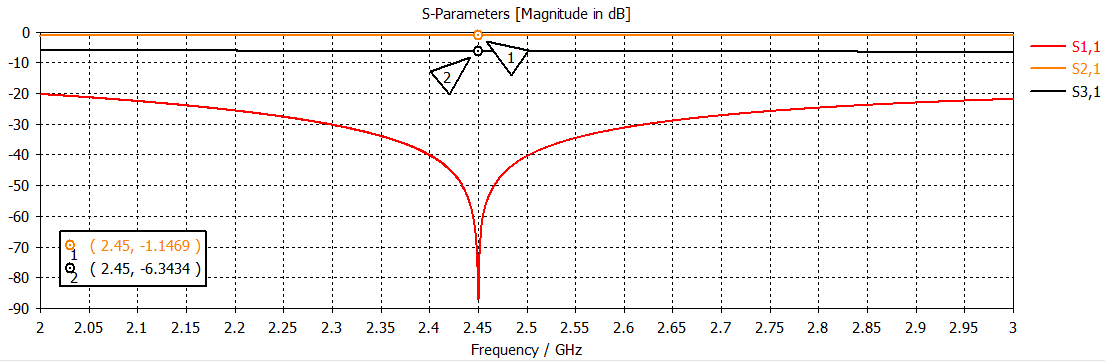
\includegraphics[scale=.6,angle=90]{p1_sec2_Smod}}\quad
	\subfloat[][\emph{Phase}]{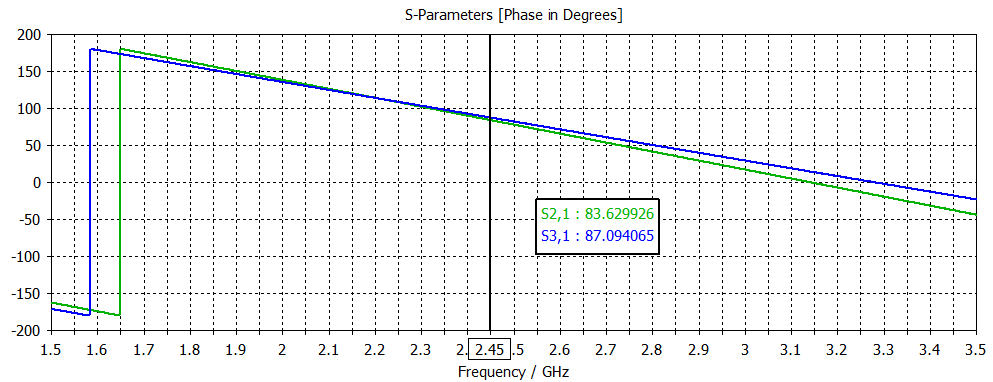
\includegraphics[scale=.6,angle=90]{p1_sec2_Sph}}\\
	\caption{Section 1 most important scattering parameters. As it appears both input matching and even power splitting are accomplished. The tapering value is t=-5.2dB, the phase shift amount to 3.94$^\circ$ (reference impedance 50$\Omega$).}.
	\label{fig:p2_sec1Scatt}
\end{figure}

\subsection{Match2 design}

As final design step another quarter-wavelength transformer is introduced. This element matches splitter2 and splitter3, R\textsubscript{out}=50$\Omega$, output impedance with the radiators' input impedance, equal to Z\textsubscript{in,patch}=120$\Omega$. Using equation (\ref{eq:p1_ZcQW}) we have:
\begin{align}
	Z_{c,M2}&=\sqrt{R_{in,M2}\cdot R_{out,M2}} \notag\\
	&=\sqrt{Z_{out}\cdot Z_{in,patch}} \notag\\
	&=\sqrt{120\Omega \cdot 50\Omega}=77.5\Omega \notag
\end{align}
The conversion from ideal microstrip to layout can be found in table \ref{tab:21_DimM2}.

\begin{table} [h]
	\label{tab:21_DimM2}
	\caption{Match2: microstrip dimensions.}
	\centering	
	\begin{tabular}{lccc} 
		\toprule
		& theoretical 			& optimized &\\
		\midrule 
		W\textsubscript{M1} 	&	1.316		&	1.212	& mm 		\\
		L\textsubscript{M1}		&	17.365		& 	17.365	& mm		\\ 
		Z\textsubscript{c,M1}	&	77.5		& 	80.45	& $\Omega$		\\
		\bottomrule
	\end{tabular}	
\end{table}

\begin{figure}[t] 
	\centering
	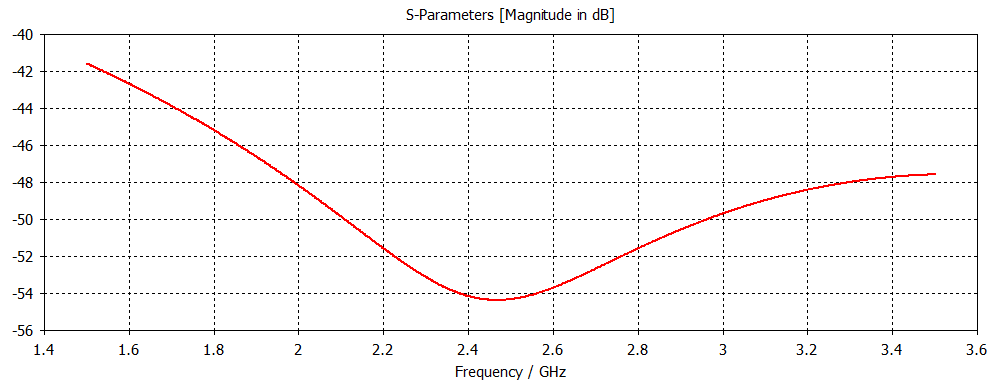
\includegraphics[scale=0.5]{p1_M2_Smod}
	\caption{Match2 return loss (reference impedance 50$\Omega$). }
	\label{fig:e1_array}
\end{figure}
\section{Problem no.2}

In order to verify and optimize the design of the BFN we decided to use \textit{CST Design Studio}, one of the various tools offered by \textit{CST Studio Suite}, which allows the user to design a microstrip network via schematic, to optimize it through the embedded optimization tool and then to create a layout of the whole project that can easily be exported in \textit{CST Microwave Studio} for further simulations.

\par\medskip
\noindent
Figure \ref{BFN_schematic} shows how a schematic looks like in \textit{CST Design Studio}. The isolated block is needed in order to assign to the structure fundamental properties such as thickness of the ground plane and dielectric constant of the substrate, while the other blocks build up the whole structure, allowing the creation of lines with assigned width and length and even bends (for example mitered) and junctions.

\begin{figure}[H]
\centering
\includegraphics[scale=0.4]{BFN_schematic.png}
\caption{BFN schematic on \textit{CST Design Studio}}
\label{BFN_schematic}
\end{figure}

\par\medskip
\noindent
As a first step the BFN has been drawn with the dimensions calculated during the design phase and then we specified that we wanted to see the S parameters at all ports (port 1 has an impedance of 50 $\Omega$, ports 2 to 5 have an impedance of 120 $\Omega$, since they take the place of the patches) as a simulation result. Next, the optimizer was set with the initial goal of tuning the S\textsubscript{11} parameter so to make it resonate at 2.45 GHz with the highest possible precision, obtaining the result shown in figure \ref{BFN_S11}.

\begin{figure}[H]
\centering
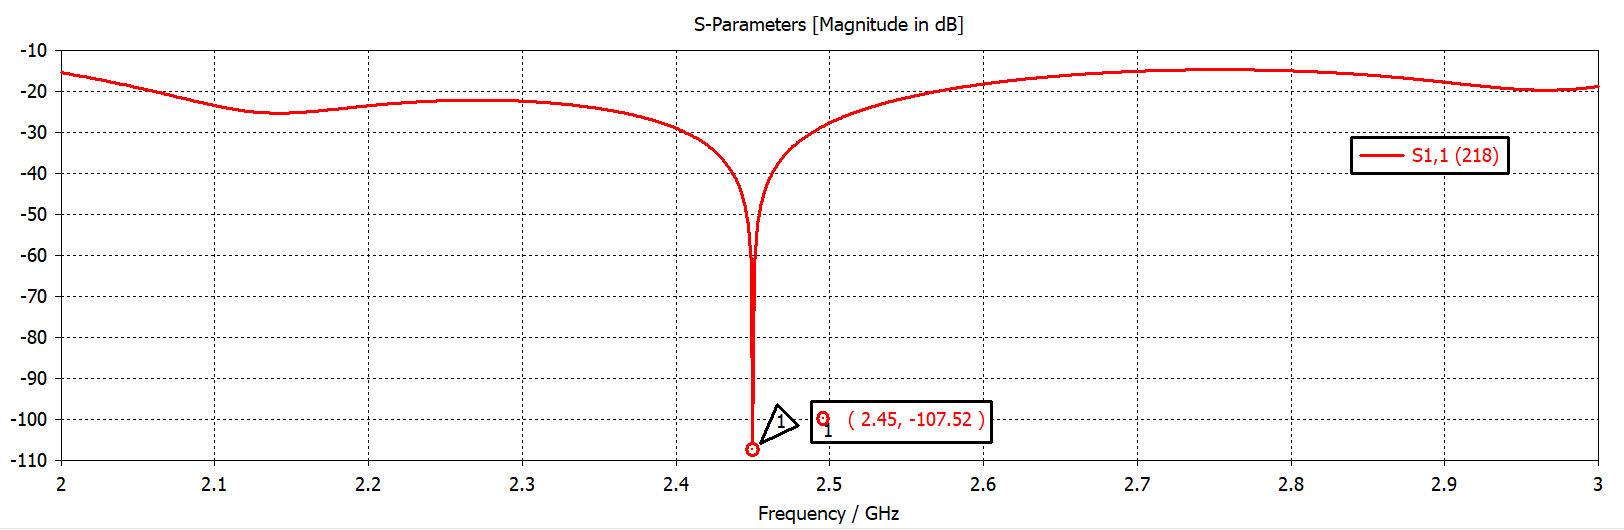
\includegraphics[scale=0.35]{BFN_S11.png}
\caption{S\textsubscript{11} parameter of our BFN}
\label{BFN_S11}
\end{figure}

\par\medskip
\noindent
As one can see, S\textsubscript{11} is pretty well shaped and furthermore the resonance at the desired frequency is strong and the obtained bandwidth is quite large.

\par\medskip
\noindent
Next step is the verification of the obtained tapering and phasing, which can be done by checking the value of the S\textsubscript{ij} parameters.

\begin{figure}[H]
\centering
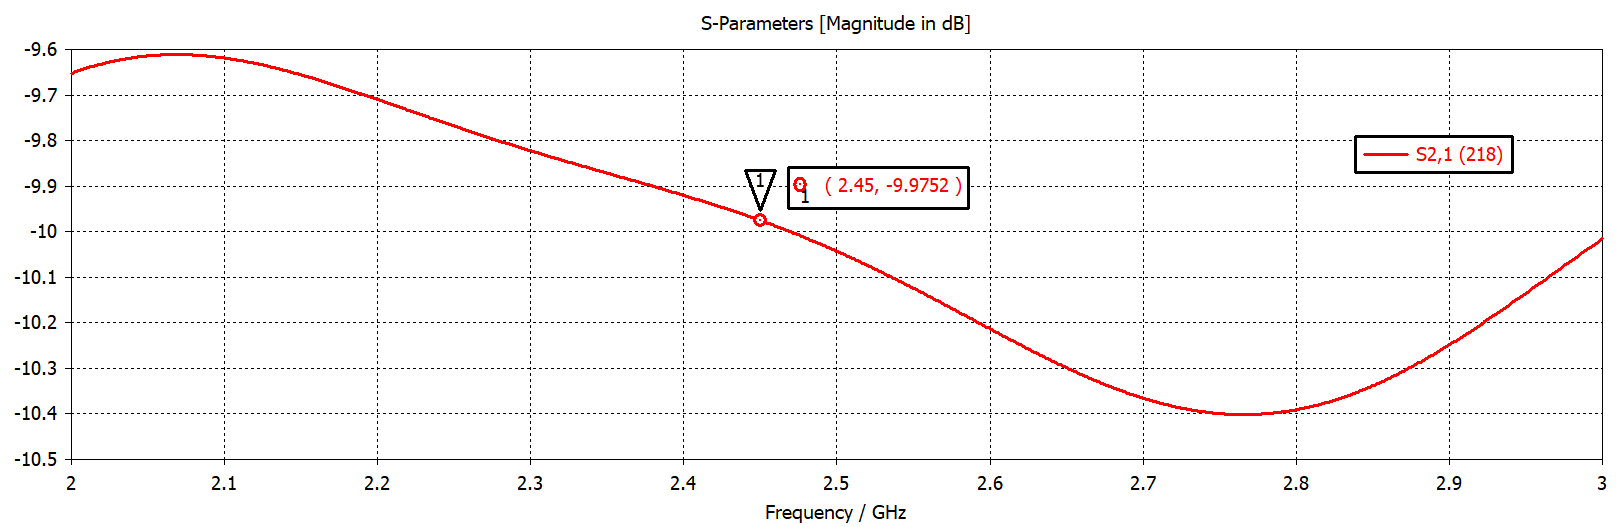
\includegraphics[scale=0.35]{S21Amp.png}
\caption{S\textsubscript{21} parameter of our BFN}
\label{S21Amp}
\end{figure}

\begin{figure}[H]
\centering
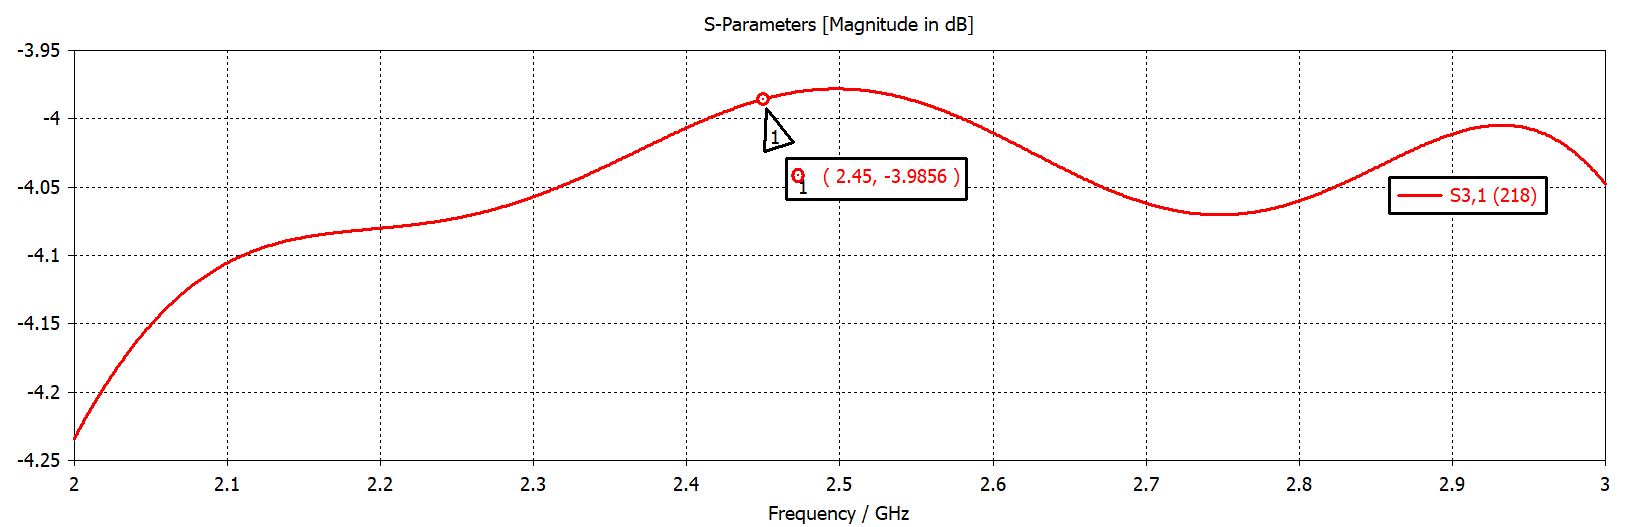
\includegraphics[scale=0.35]{S31Amp.png}
\caption{S\textsubscript{31} parameter of our BFN}
\label{S31Amp}
\end{figure}

\begin{figure}[H]
\centering
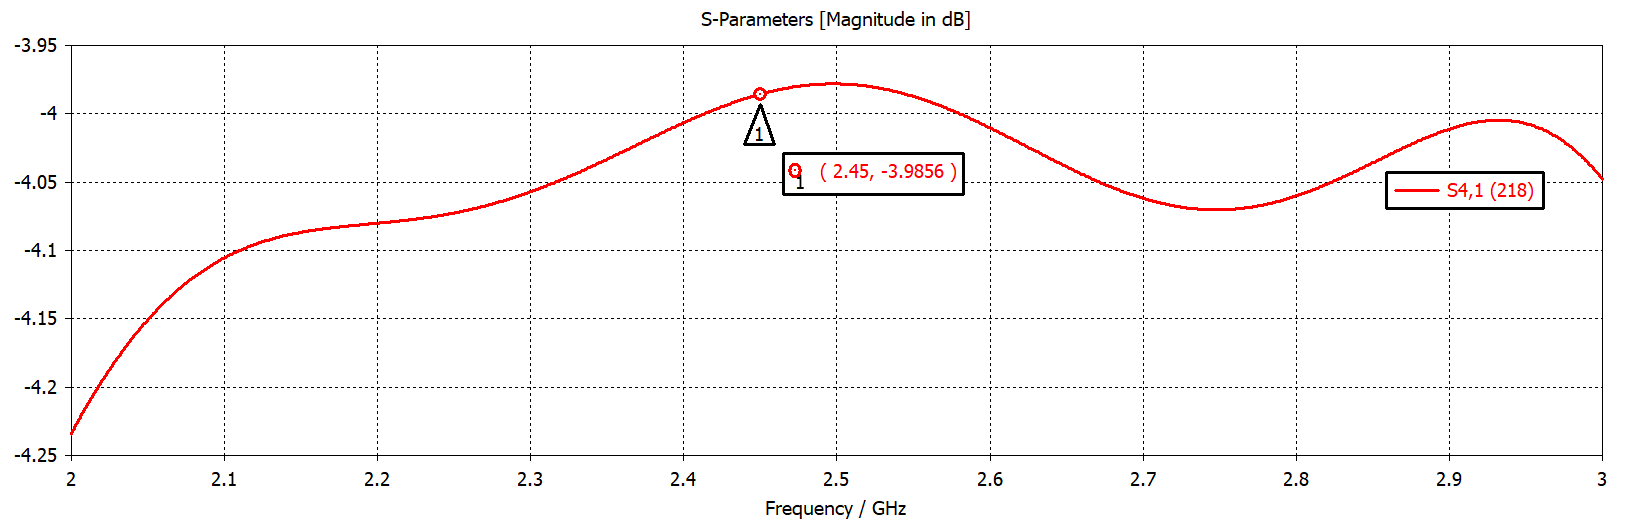
\includegraphics[scale=0.35]{S41Amp.png}
\caption{S\textsubscript{41} parameter of our BFN}
\label{S41Amp}
\end{figure}

\begin{figure}[H]
\centering
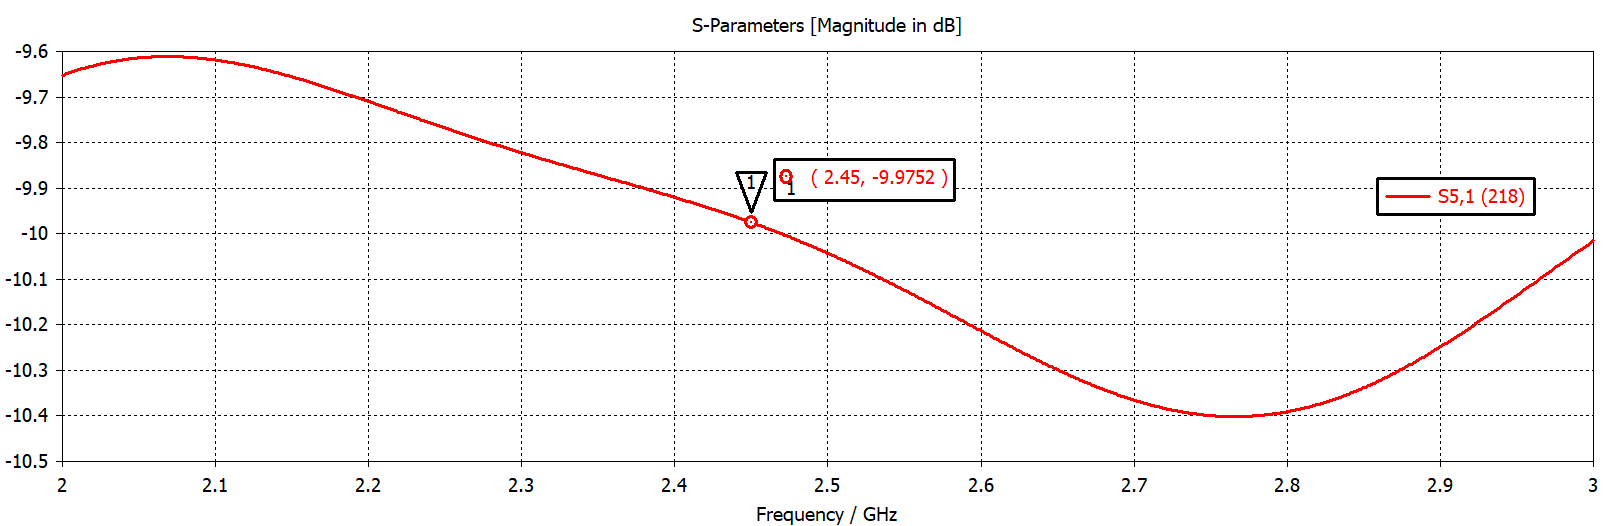
\includegraphics[scale=0.35]{S51Amp.png}
\caption{S\textsubscript{51} parameter of our BFN}
\label{S51Amp}
\end{figure}

\par\medskip
\noindent
The power ratio between the central elements of the array (ports 3 and 4) and the edge ones (ports 1 and 5) turns out to be 5.98 dB.

\par\medskip
\noindent
Last but not least, we have to verify that the phase shift between the output ports is as close as possible to 0.

\begin{figure}[H]
\centering
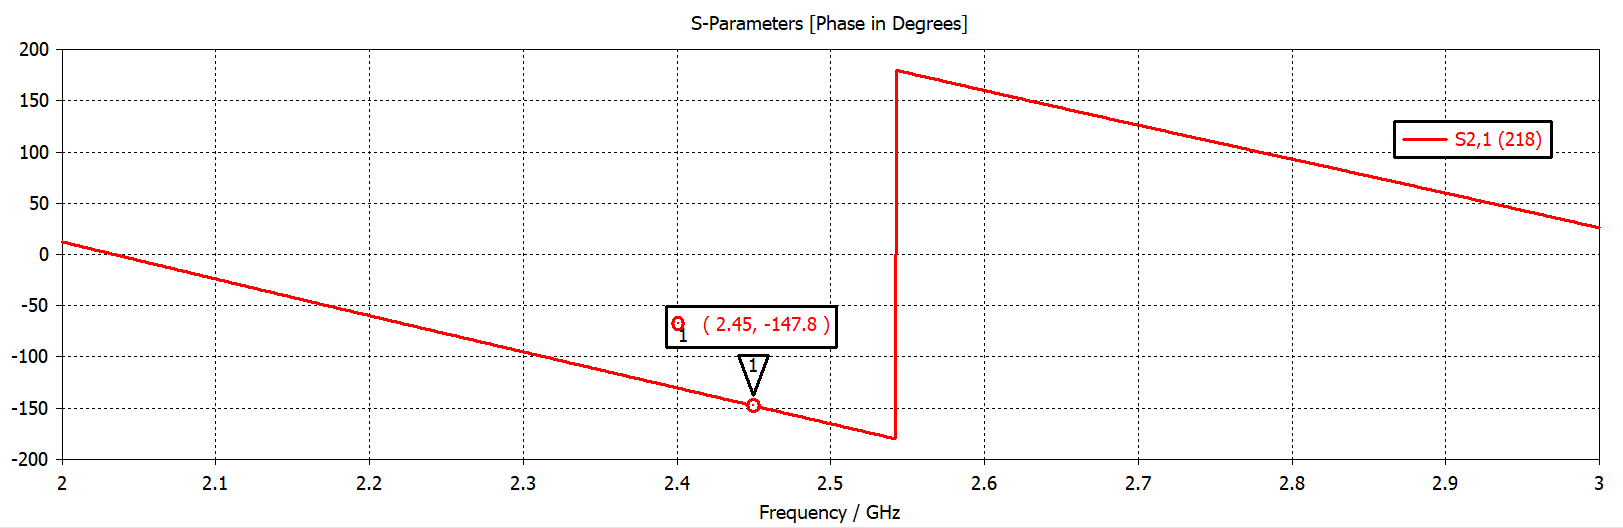
\includegraphics[scale=0.35]{S21p.png}
\caption{S\textsubscript{21} parameter (phase), coinciding with S\textsubscript{51}}
\label{S21phase}
\end{figure}

\begin{figure}[H]
\centering
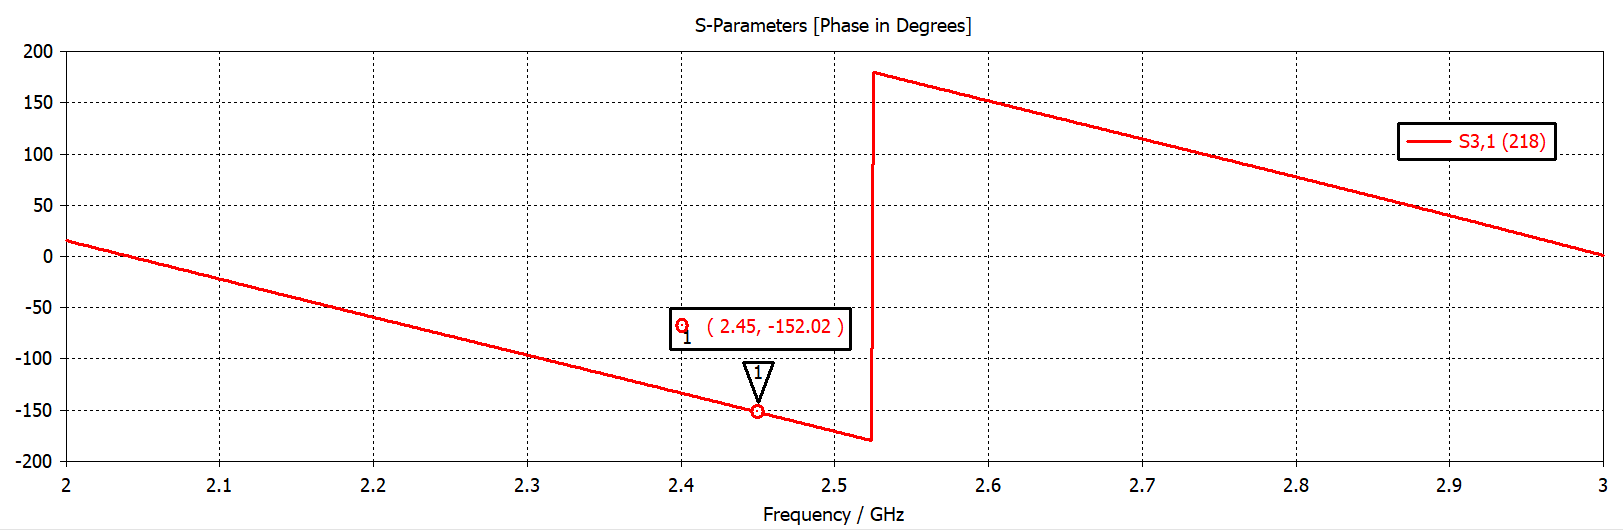
\includegraphics[scale=0.35]{S31p.png}
\caption{S\textsubscript{31} parameter (phase), coinciding with S\textsubscript{41}}
\label{S31phase}
\end{figure}

\par\medskip
\noindent
The phase difference between center and edge elements is around 4\textsuperscript{$\circ$}. A simulation of the complete structure in \textit{Microwave Studio} will tell us whether this lack of precision will affect the behavior of the array a lot or it will result either way to be broadside, as expected.

\par\medskip
\noindent
In order to have a visual impact of what the schematic is translated into in terms of layout, figure \ref{layout} shows the resulting structure.

\begin{figure}[H]
\centering
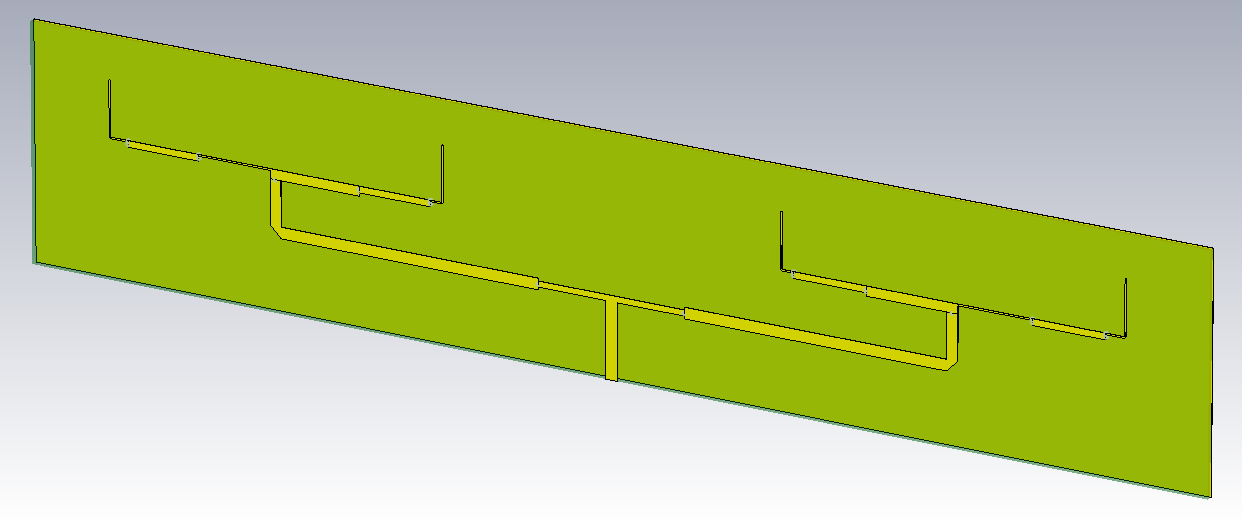
\includegraphics[scale=0.45]{layout.png}
\caption{How our BFN looks like}
\label{layout}
\end{figure}

\par\medskip
\noindent
Unfortunately, if till this point the simulations seemed to be very encouraging, we realized that when trying to transfer the design on \textit{CST Microwave Studio} they were not so good: the resonance was not as precise as we'd have expected and neither was the tapering. Furthermore, if using the optimizer turned out to be a very useful tool when using \textit{Design Studio}, things are not so easy in \textit{Microwave Studio}, where the high density of the mesh needed in order to obtain reliable results makes the simulation time very long. Due to these reasons we began from scratch, trying to build up the single components of the BFN separately. As previously described the power splitters seem to work on their own, giving the correct power ratio and phasing, but even in this case we were not able to put them together obtaining a satisfactory result, nor we managed to optimize the results on the base of what previously obtained. The reasons are multiple: long simulation time if the mesh is dense and low reliability if, with the aim of reducing the simulation time to allow for optimization, one uses a larger meshgrid, very high precision of the optimizer, which specifies a lot of digits (which has no sense if one thinks about the specifications one should give the producer in order to print the antenna). Furthermore: every curve introduces a non ideality and even the simple lines are not easy to tune all together to the correct impedance value. Simulations were carried out both with discrete face ports (whose reference impedance can be specified by the user) and with waveguide ports, but in both case we were unable to tune the BFN perfectly.

\par\medskip
\noindent
We also tried to simulate the behavior of the BFN when attached to the patches, but, since the tapering was not the good one we had hoped for, the SLL wasn't completely tuned on the -20 dB level either. Good notes are the fact that the radiated field happened to be broadside, meaning that the phasing, at least, was correct, and that the resonce frequency, even if not perfect, happened to be more precise in this case.
\section{Problem no.3}
In this last part the aim is to verify the radiating element behavior, starting from the single patch and arriving to the complete array. For the patch antenna we use the one we designed for the second laboratory, that are described in the following image *.
\begin{figure}[H]
	\centering
	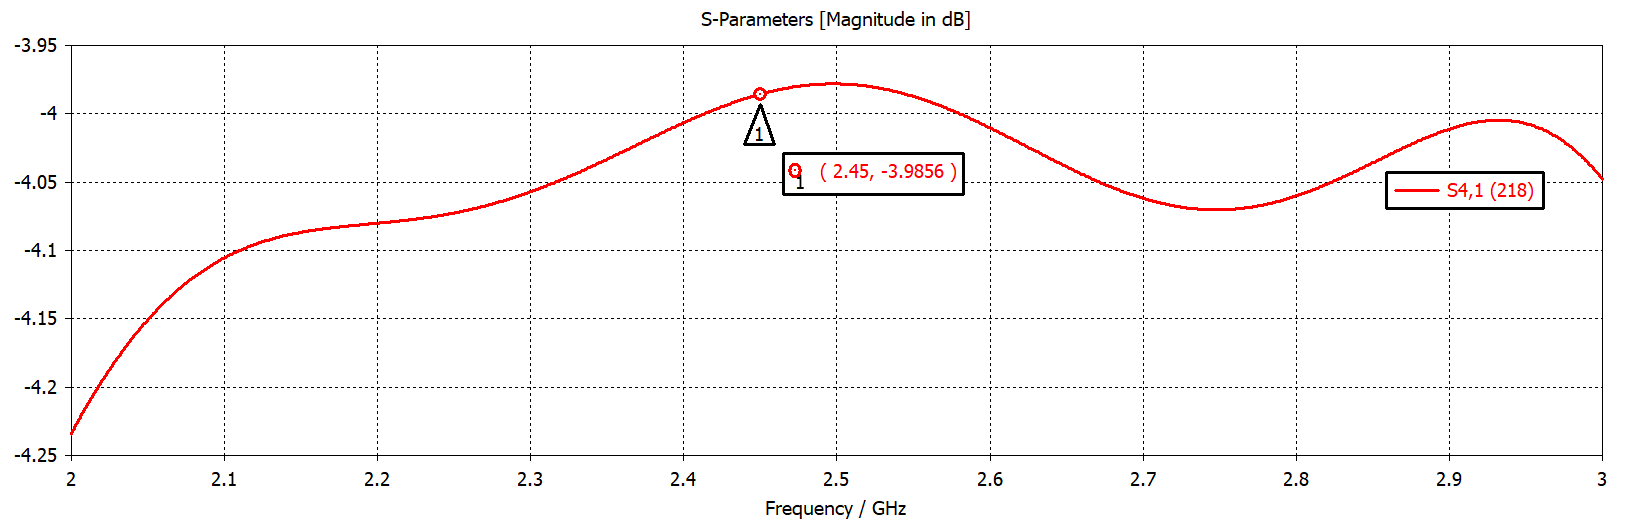
\includegraphics[scale=0.35]{S41Amp.png}
	\caption{S\textsubscript{41} parameter of our BFN}
	\label{S41Amp}
\end{figure}

\paragraph{single antenna} First of all we analyze the single antenna itself, so that we control it resonates at the correct frequency with our feeding. We use a very short line with characteristic impedance close to the patch output one, in order to simulate the effective feeding that will be implemented with the beam forming network. This choice is made also to minimize the contribution due to the mismatching of the load the line, and in fact the length of the microstrip feeding is much less than the guided wavelength at the resonance frequency.
\begin{figure}[H]
	\centering
	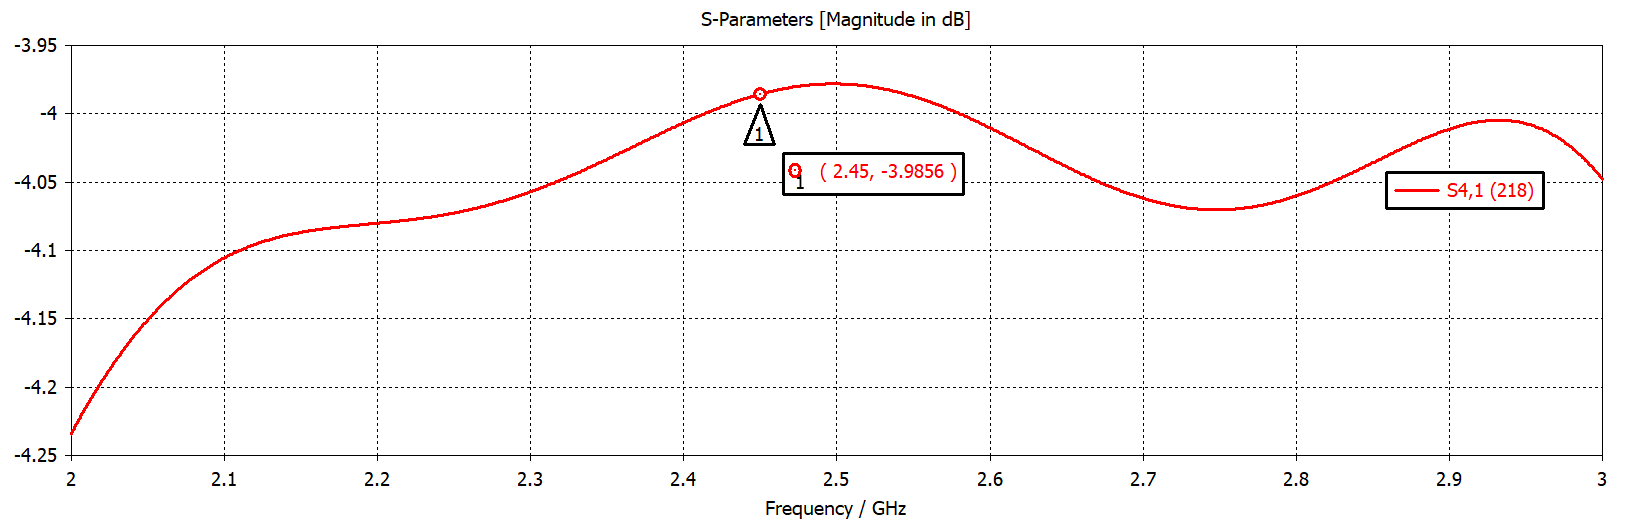
\includegraphics[scale=0.35]{S41Amp.png}
	\caption{S\textsubscript{41} parameter of our BFN}
	\label{S41Amp}
\end{figure}
The initial values shows a behavior not optimal for our situation, and so we have to made a little tuning (not too much because probably the inter element coupling will influence the scattering parameters and it will be required another optimization). *comments*

\paragraph{multiple antennas} Composing the array with those antennas we can have a first simulation of the complete radiating element, and so we can make some considerations. The bigger issue in particular are the resonance frequency, which due to the inter elements coupling (as expected) are deviated from the single antenna case. In particular the resonance frequency results shifted of few hundreds of megahertz upward, movement that we have to take in mind in order to re-design a similar patch antenna complying better with the specifications.
\begin{figure}[H]
	\centering
	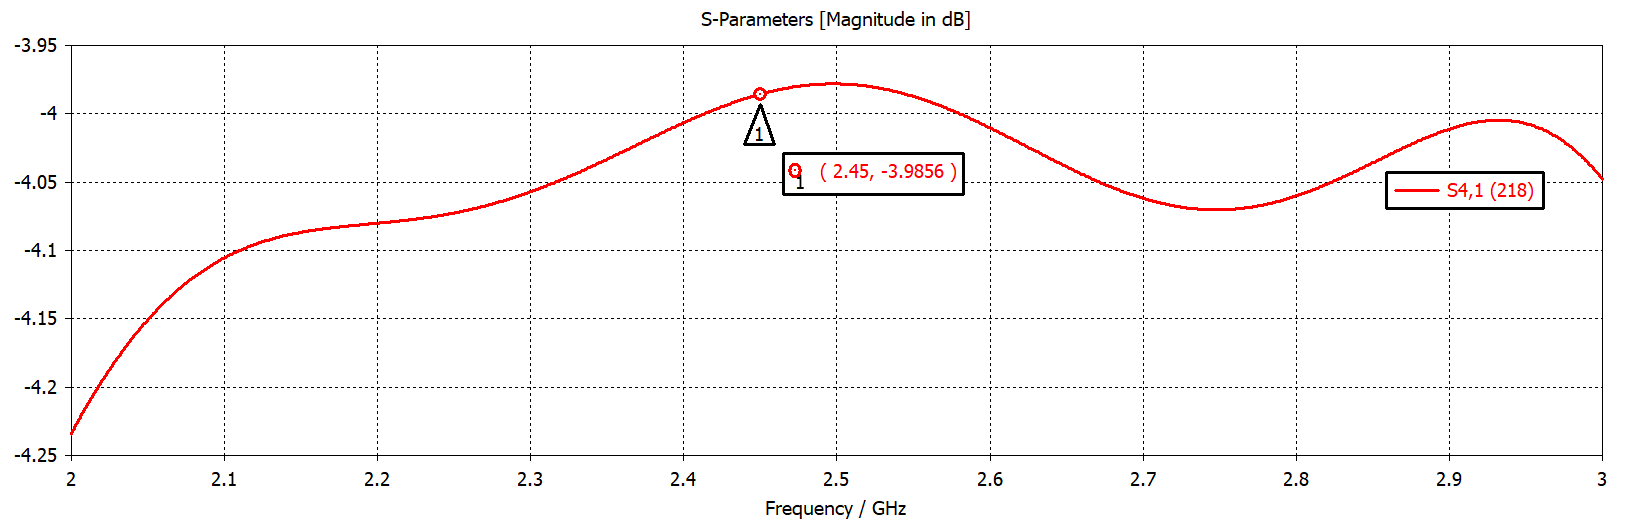
\includegraphics[scale=0.35]{S41Amp.png}
	\caption{S\textsubscript{41} parameter of our BFN}
	\label{S41Amp}
\end{figure}
Simulating the four antennas with their entering ports we have a total number of 16 scattering parameters, which are not so easy to handle in order to find the load seen from the beam forming network point of view and optimize it. Because we use a constant tapering for the antennas feeding we can combine the results of this simulation and find only four scattering parameters describing the reflection coefficient of each port. This way we can also find the relative impedance, so that in our particular case of feeding we can evaluate precisely the active impedance of the antennas. The value founded this way are showed in the figures * and *
\begin{figure}[H]
	\centering
	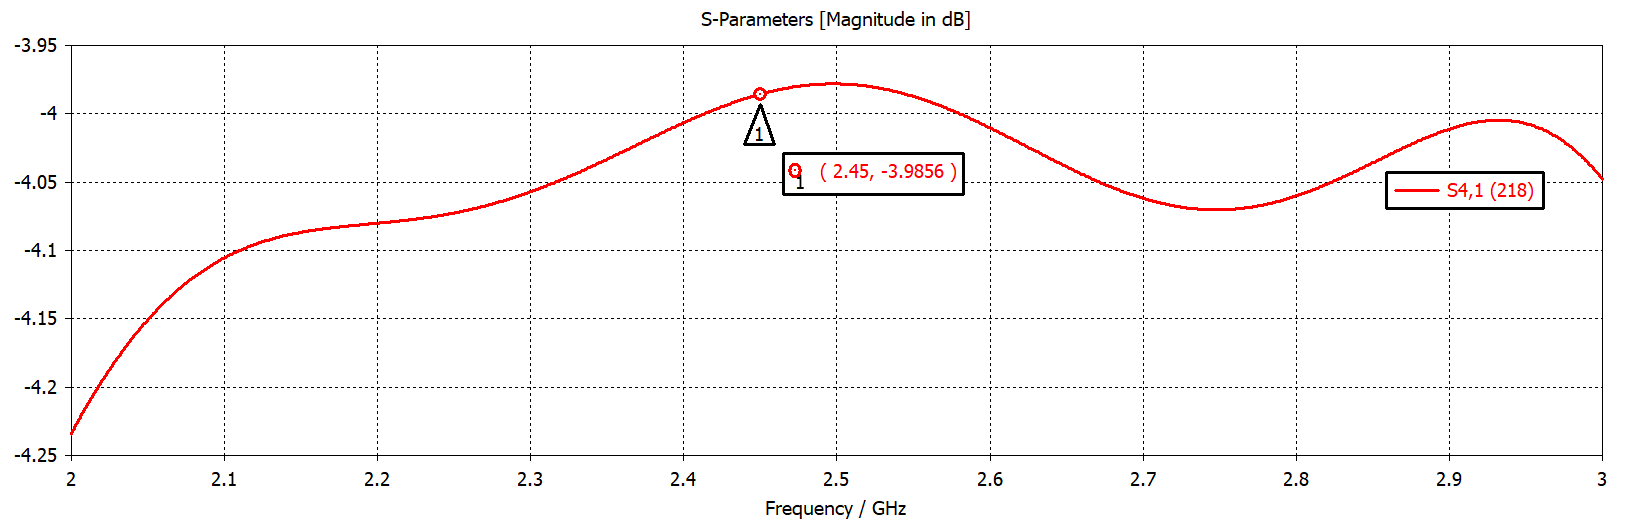
\includegraphics[scale=0.35]{S41Amp.png}
	\caption{S\textsubscript{41} parameter of our BFN}
	\label{S41Amp}
\end{figure}
Cause of the symmetry of the structure we have that the impedance of the external elements slightly differs from the internal one, but as reported in the graph * the difference is negligible.

\paragraph{array factor} The last pass is to consider the radiation pattern, which is first of all evaluated with a far field monitor, and after that is exported and elaborated in Matlab in order to verify the correct behavior of the array factor. For this calculation we need also the far field radiation of the single patch antenna, which must be used as a punctual divider for the array far field (remembering the relation *formula*).
\begin{lstlisting}
% ** preset of all the variables **
alpha=linspace(0,2*pi,10000);
\end{lstlisting}
The result of this calculation is the array factor printed in figure *, which respect all the initial requirements.
\begin{figure}[H]
	\centering
	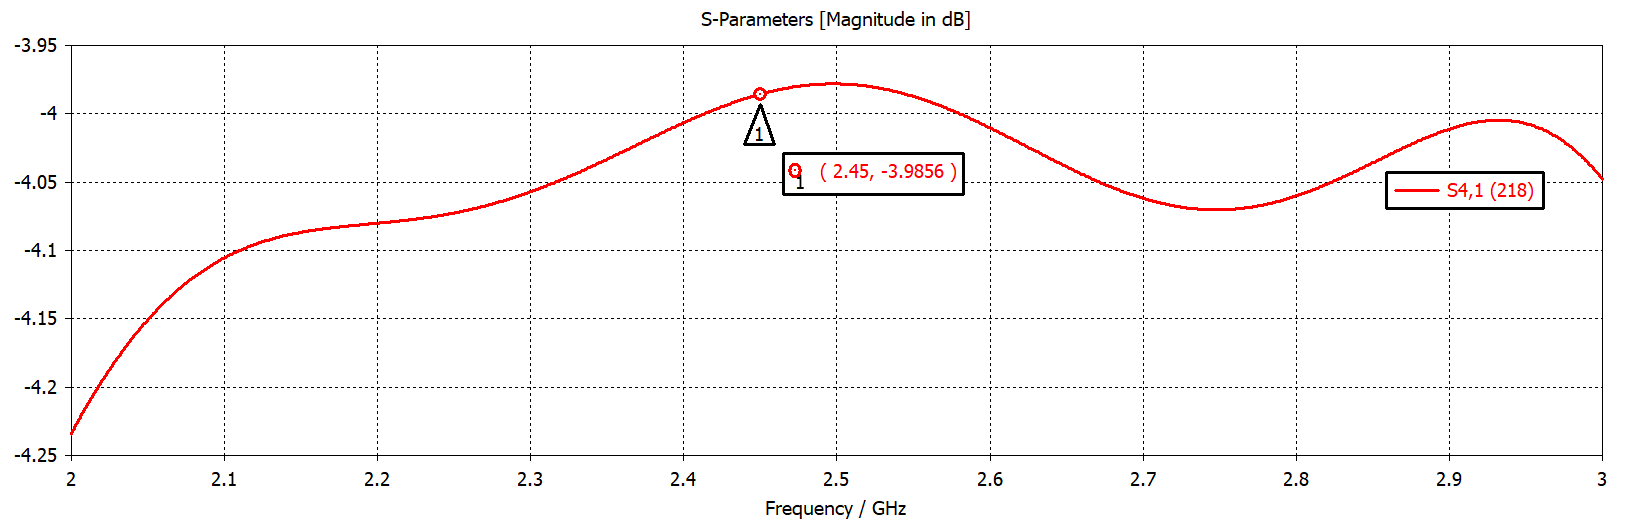
\includegraphics[scale=0.35]{S41Amp.png}
	\caption{S\textsubscript{41} parameter of our BFN}
	\label{S41Amp}
\end{figure}

\section{EXAMPLE, PLEASE DELETE ME}
following an example of frame for Matlab
\begin{lstlisting}
% ** preset of all the variables **
alpha=linspace(0,2*pi,10000);
\end{lstlisting}
\paragraph{things to write} are divided in paragraphs
\subparagraph{or subparagraphs} like this
\end{document}
